\begin{center}
\Huge
Niveaukurver og snitkurver
\end{center}

\section*{Niveaukurver}
\stepcounter{section}

Det kan være en fordel at betragte en funktion af to variable som et landskab, hvor funktionsværdien $f(x,y)$ er højden af landskabet og $x$-koordinaten er breddegraden og $y$-koordinaten er længdegraden. 
\begin{exa}
	På Fig. \ref{fig:nedboer} ses den summerede nedbørsmængde i Danmark fra d. 26.-28. august. 
	Som funktion af bredde- og længdegraderne $x$ og $y$ kan vi bestemme nedbørsmængden
	$N(x,y)$. 
	\begin{figure}[H]
		\centering
		\includegraphics[width=0.6\textwidth]{Billeder/nedboer.png}
		\caption{Summeret nedbør d. 26.-28. august}
		\label{fig:nedboer}
	\end{figure}
\end{exa} 

I stedet for at tegne en figur i 3d, så kan det være en fordel at tegne en figur i $xy$-planen, hvor kurver med bestemte funktionsværdier tegnes ind. Dette kan give et bedre overblik over forløbet for grafen for funktionen. Sådanne kurver kaldes for \textit{niveaukurver}.
\begin{defn}[Niveaukurver]
	Lad $f: \mathbb{R} \times \mathbb{R} \to \mathbb{R}$ være en funktion af to variable, og 
	$k$ en konstant. Så kaldes punktmængden $\{(x,y,f(x,y)) \mid f(x,y) = k\}$ for en 
	niveaukurve for $f$. 
\end{defn}
Definitionen for en niveaukurve kan virke lidt abstrakt, og den er klart nemmest forstået gennem eksempler. 
\begin{exa}
	På Fig. \ref{fig:isobar} kan vi se niveaukurver for en funktion, der for et koordinatsæt $(x,y)$ giver lufttrykket et givent sted i Europa d. 7 septemper 2022 (prognose). 
	Disse niveaukurver kaldes for isobarer, og deler Europa op i intervaller af lufttryk. Det er typisk med sådanne niveaukurver at højtryk og lavtryk præsenteres.
	\begin{figure}[H]
		\centering
		\includegraphics[width=0.6\textwidth]{Billeder/Lufttryk.png}
		\caption{Lufttryk over Europa d. 7. september kl 20:00 (prognose).}
		\label{fig:isobar}
	\end{figure}
\end{exa}

\begin{exa}
	Vi kan bestemme niveaukurver for paraboloiden, der er graf for funktionen $f$ givet ved
	\begin{align*}
		f(x,y) = x^2+y^2.
	\end{align*} 
	Grafen samt niveaukurver for $f$ kan ses af Fig. \ref{fig:paraboloide}
	\begin{figure}[H]
		\centering
		\includegraphics[width=0.45\textwidth]{Billeder/Paraboloide.png}
		\includegraphics[width=0.45\textwidth]{Billeder/niveauparabol.png}
		\caption{Paraboloide med niveaukurver.}
		\label{fig:paraboloide}
	\end{figure}
	Det kan godt tyde på, at niveaukurverne er cirkler. Det er også tilfældet. Betragter vi en niveaukurve, der består af punktmængden $(x,y)$, så $f(x,y) = k$, så vil vi have
	\begin{align*}
		k = x^2 + y^2,
	\end{align*}
	men dette er netop ligningen for en cirkel med centrum i $(0,0)$ og radius $\sqrt{k}$. 
\end{exa}

\section*{Snitkurver}
\stepcounter{section}

Til at analysere funktioner af to variable kan vi også bruge \textit{snitkurver}. På samme måde som niveaukurver er vandrette snit af grafen for funktionen $f$, så vil snitkurver være lodrette snit typisk langs enten $yz$- eller $xz$-planen. Vi definerer snitkurver på følgende vis.
\begin{defn}[Snitkurver]
	Lad $f:\mathbb{R}\times \mathbb{R} \to \mathbb{R}$ være en funktion af to variable. For en konstant $k\in\mathbb{R}$ defineres punktmængden
	\begin{align*}
		\{(k,y,f(k,y))\}
	\end{align*}
	som snitkirven i $x$-retningen, og punktmængden
	\begin{align*}
		\{(x,k,f(x,k))\}
	\end{align*}
	defineres som snitkurven i $y$-retningen. 
\end{defn}

\begin{exa}
	Vi betragter igen funktionen $f$ givet ved
	\begin{align*}
		f(x,y) = x^2 + y^2.
	\end{align*}
	Vi vælger at betragte snittet langs  henholdsvist $x$- og $y$-aksen med $k= 2$. Dette giver os snitfunktionerne
	\begin{align*}
		h_y(x) = f(x,2) = x^2+4,
	\end{align*}
	og 
	\begin{align*}
		h_x(y) = f(2,y) = y^2+4.
	\end{align*}
	Snitkurverne er graferne for disse funktioner, og det kan ses, at snitkurverne er parabler. Snitkurverne kan ses af Fig. \ref{fig:snit}	
	\begin{figure}[H]
		\centering
		\resizebox{0.45\textwidth}{!}{
		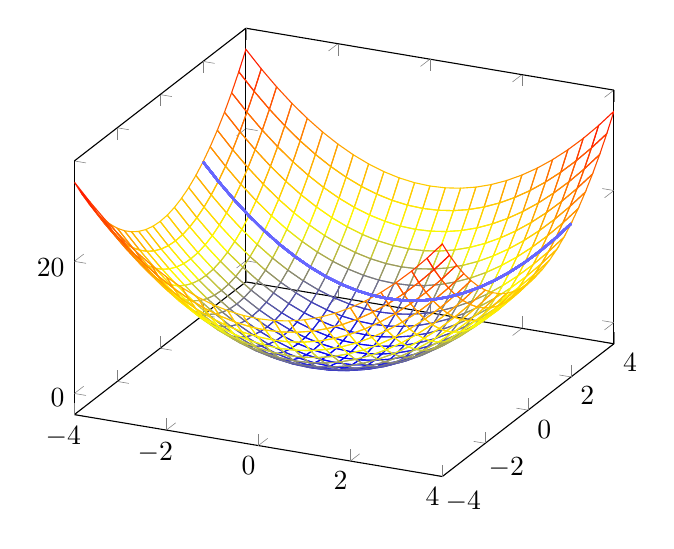
\begin{tikzpicture}
			\begin{axis}[xmin = -4, xmax = 4,ymin = -4, ymax = 4]
				\addplot3[domain = -4:4, domain y = -4:4, mesh] {x^2+y^2};
				\addplot3[variable = t, domain = -4:4, mesh, color = blue!60, thick ]  (t,2,{t^2+4});
			\end{axis}
		\end{tikzpicture}
		}
		\resizebox{0.45\textwidth}{!}{
		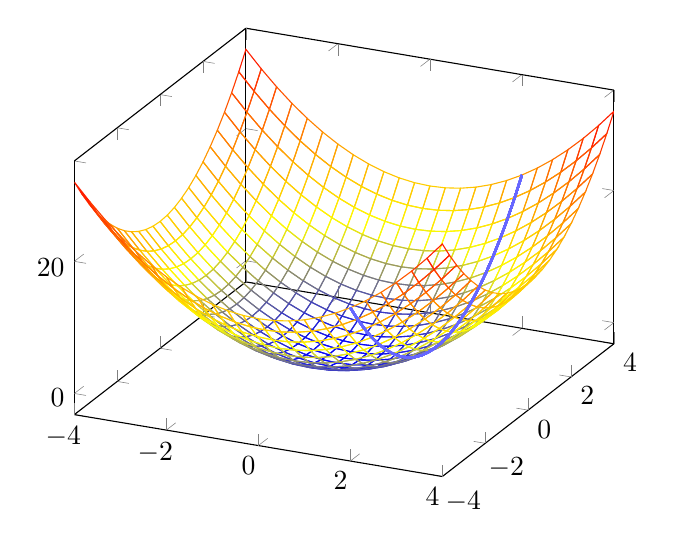
\begin{tikzpicture}
			\begin{axis}[xmin = -4, xmax = 4,ymin = -4, ymax = 4]
				\addplot3[domain = -4:4, domain y = -4:4, mesh] {x^2+y^2};
				\addplot3[variable = t, domain = -4:4, mesh, color = blue!60, thick ]  (2,t,{t^2+4});
			\end{axis}
		\end{tikzpicture}
		}
		\caption{Snitkurver for paraboloide.}
		\label{fig:snit}
	\end{figure}
\end{exa}

\section*{Opgave 1}
Følgende grafer for funktioner af to variable er givet samt deres niveaukurver. Par graferne med niveaukurverne.
\begin{center}
\includegraphics[width=0.25\textwidth]{Billeder/xy.png}
\includegraphics[width=0.25\textwidth]{Billeder/cosxyniveau.png}\\
\includegraphics[width=0.25\textwidth]{Billeder/cossin.png}
\includegraphics[width=0.25\textwidth]{Billeder/planeniveau.png} \\
\includegraphics[width=0.25\textwidth]{Billeder/plane.png}
\includegraphics[width=0.25\textwidth]{Billeder/cosxxniveau.png}\\
\includegraphics[width=0.25\textwidth]{Billeder/sqrt.png}
\includegraphics[width=0.25\textwidth]{Billeder/hyperbelniveau.png}\\
\includegraphics[width=0.25\textwidth]{Billeder/xdivy.png}
\includegraphics[width=0.25\textwidth]{Billeder/xyniveau.png}\\
\includegraphics[width=0.25\textwidth]{Billeder/cosxy.png}
\includegraphics[width=0.25\textwidth]{Billeder/sqrtniveau.png}\\
\includegraphics[width=0.25\textwidth]{Billeder/cosxx.png}
\includegraphics[width=0.25\textwidth]{Billeder/xdivyniveau.png}\\
\includegraphics[width=0.25\textwidth]{Billeder/hyperbel.png}
\includegraphics[width=0.25\textwidth]{Billeder/cossinniveau.png}\\
\end{center}


\section*{Opgave 2}
En paraboloide er givet ved funktionen 
\begin{align*}
	f(x,y) = x^2+y^2
\end{align*}
\begin{enumerate}[label=\roman*)]
	\item Niveaukurven for $f$ i højden $k = 4$ bestemmer en cirkel. Bestem radius og centrum for denne cirkel.
	\item Afgør, om punktet $(0,4,16)$ ligger på niveaukurven i højden $k=16$.
\end{enumerate}

\section*{Opgave 3}
En paraboloide er givet ved funktionen
\begin{align*}
	f(x,y) = x^2+y^2+2(x+y)+4.
\end{align*}
\begin{enumerate}[label=\roman*)]
	\item Niveaukurven for $f$ i højden $k=14$ bestemmer en cirkel. Bestem radius og centrum for denne cirkel. 	
\end{enumerate}

\section*{Opgave 4}
\begin{enumerate}[label=\roman*)]
	\item Bestem en snitkurve for følgende funktioner i planen $y=3$.
	\begin{align*}
	&1) \ f(x,y) = x^2+y^2  &&2) \  f(x,y) = x^3-y^2+1,\\
	&3) \ f(x,y) = \cos(x)+\sin\left(\pi\frac{y}{3}\right)  &&4) \  f(x,y) = \sqrt{3y} + 3x^5.
	\end{align*}
\end{enumerate}

\section*{Opgave 5}

\begin{enumerate}[label=\roman*)]
	\item Bestem en snitkurve for følgende funktioner i planen $x=1$.
	\begin{align*}
	&1) \ f(x,y) = x^2-y^2  &&2) \  f(x,y) = \frac{x}{y},\\
	&3) \ f(x,y) = \sqrt{xy}  &&4) \  f(x,y) = x.
	\end{align*}
\end{enumerate}

\section*{Opgave 6}
Vi har set, at den øvre halvkugle af en kugle med centrum i $C(0,0,0)$ og radius $r$ kan beskrives ved grafen for funktionen $f$ givet ved
\begin{align*}
	f(x,y) = \sqrt{r^2-x^2-y^2}.
\end{align*}
Vis, at niveaukurverne for $f$ er cirkler, og bestem centrum og radius for disse cirkler givet en højde $k$ for niveaukurven. 